\documentclass[a4paper]{ctexrep}
\usepackage{ctex}
\usepackage{times}
\usepackage{setspace}
\usepackage{fancyhdr}
\usepackage{graphicx}
\usepackage{wrapfig}
\usepackage{array}  
\usepackage{fontspec,xunicode,xltxtra}
\usepackage{titlesec}
\usepackage{titletoc}
\usepackage[titletoc]{appendix}
\usepackage[top=30mm,bottom=30mm,left=20mm,right=20mm]{geometry}
\usepackage{listings}
\usepackage{enumerate}
\usepackage{algorithm}
\usepackage{algorithmicx}
\usepackage{algpseudocode}
\usepackage{color}
\usepackage{appendix}



\definecolor{codegreen}{rgb}{0,0.6,0}
\definecolor{codegray}{rgb}{0.5,0.5,0.5}
\definecolor{codepurple}{rgb}{0.58,0,0.82}
\definecolor{backcolour}{rgb}{0.95,0.95,0.92}




\setmainfont{TeX Gyre Pagella}
\floatname{algorithm}{伪代码}
\renewcommand{\algorithmicrequire}{\textbf{Input:}}
\renewcommand{\algorithmicensure}{\textbf{Output:}}
\newcommand{\numofexp}{五}

%---------------------------------------------------------------------
%	页眉页脚设置
%---------------------------------------------------------------------
\fancypagestyle{plain}{
	\pagestyle{fancy}      %改变章节首页页眉
}

\pagestyle{fancy}
\lhead{\kaishu~TCP/IP课程实验报告~}
\rhead{\kaishu~1030616134~尹达恒~}
\cfoot{\thepage}

%---------------------------------------------------------------------
%	章节标题设置
%---------------------------------------------------------------------
\titleformat{\chapter}{\centering\zihao{-1}\heiti}{实验\numofexp}{1em}{}
\titlespacing{\chapter}{0pt}{*0}{*6}

%---------------------------------------------------------------------
%	目录页设置
%---------------------------------------------------------------------
\titlecontents{chapter}[0em]{\songti\zihao{-4}}{\thecontentslabel\ }{}
{\hspace{.5em}\titlerule*[4pt]{$\cdot$}\contentspage}
\titlecontents{section}[2em]{\vspace{0.1\baselineskip}\songti\zihao{-4}}{\thecontentslabel\ }{}
{\hspace{.5em}\titlerule*[4pt]{$\cdot$}\contentspage}
\titlecontents{subsection}[4em]{\vspace{0.1\baselineskip}\songti\zihao{-4}}{\thecontentslabel\ }{}
{\hspace{.5em}\titlerule*[4pt]{$\cdot$}\contentspage}

\ctexset {
	chapter = {
		name = {实验},
		number = {\numofexp},
	},
	section = {
		number = \arabic{section},
		format = \Large\bfseries,
	},
	subsection = {
		number = \arabic{section}.\arabic{subsection},
	}
}

\begin{document}
%---------------------------------------------------------------------
%	封面设置
%---------------------------------------------------------------------
\begin{titlepage}
	\begin{center}
    
\includegraphics[width=0.9\textwidth]{figure//Njust.png}\\
    \vspace{10mm}
    \textbf{\zihao{2}\kaishu{ 物联网工程学院}}\\[0.8cm]
    \textbf{\zihao{2}\kaishu{ TCP/IP课程实验报告}}\\[3cm]
	\vspace{\fill}
	\setlength{\extrarowheight}{3mm}
	{\songti\zihao{3}	
		\begin{tabular}{rl}
			
			{\makebox[4\ccwd][s]{班\qquad 级:}}& ~\kaishu 物联1601\\
			
			{\makebox[4\ccwd][s]{姓\qquad 名:}}& ~\kaishu 尹达恒 \\ 
			
			{\makebox[4\ccwd][s]{学\qquad 号:}}& ~\kaishu 1030616134 \\ 
			
			{\makebox[4\ccwd][s]{指导老师:}} & ~\kaishu 马君霞\\ 
			
		\end{tabular}
	}\\[2cm]
	\vspace{\fill}
	\zihao{4}
	2018\textasciitilde 2019第一学期\\
	\today
	\end{center}	
\end{titlepage}



%---------------------------------------------------------------------
%  目录页
%---------------------------------------------------------------------
\tableofcontents % 生成目录
%---------------------------------------------------------------------
%  实验一
%---------------------------------------------------------------------
\chapter{基于对话框界面的消息发送应用程序}
\begin{spacing}{1.5}
\songti\zihao{-4}
\section{实验目的及要求}
\begin{itemize}
	\item 了解和掌握基于对话框的网络编程方法和界面设计工具;
	\item 学习在C\#环境下,基于C\#Windows窗体的编程,编写一个基于对话框界面的消息发送应用程序;
	\item 掌握从对话框界面输入IP地址的方法,以及添加类变量的方法。
\end{itemize}
\section{实验环境}
\begin{itemize}
	\item 操作环境:Windows 10;
	\item 编程环境:Visual Studio 2015;
	\item 程序原理:Socket网络程序设计
	\item 程序使用Visual C\#下的“Windows窗体应用程序”。
\end{itemize}
\section{实验内容及步骤}
\subsection{服务器端程序}
该程序中通信协议使用的是面向连接的TCP协议(SOCK\_STREAM)。服务器端的IP地址使用系统指定的IP地址,端口号在程序中指定为2000,用符号常量来定义。
\begin{itemize}
	\item 调试环境:Visual Stdio 2015
	\item 服务器IP地址:由系统指定
	\item 服务器端口号:2000
	\item 程序核心文件:TCPserver5/Program.cs(附录\ref{appendix}-\ref{TCPserver5/Program.cs})、TCPserver5/Form1.cs(附录\ref{appendix}-\ref{TCPserver5/Form1.cs})
	\item 程序功能:点击“准备发送”按钮后服务器端开始接收用户请求,当有客户提出连接请求时,在端口2000与客户端进行TCP连接,连接成功后,点击“发送”按钮时读取文本框中的字符串向客户端进行发送,或点击“退出”按钮关闭连接。
\end{itemize}
\subsection{客户端程序}
\begin{itemize}
	\item 调试环境:Visual Stdio 2015
	\item 客户IP地址和端口:由系统指定
	\item 程序核心文件:TCPclient5/Program.cs(附录\ref{appendix}-\ref{TCPclient5/Program.cs})、TCPclient5/Form1.cs(附录\ref{appendix}-\ref{TCPclient5/Form1.cs})
	\item 程序功能:点击“连接”按钮后客户端程序读取IP文本框中的服务器IP地址并向服务器提出TCP连接的请求,当连接建立后,点击“接收”按钮从服务器的端口2000接收数据并显示在文本框中,或点击“退出”按钮关闭连接。
\end{itemize}
\subsection{本机回环测试}
\begin{itemize}
	\item 测试环境:Visual Studio 2015
	\item 测试步骤:
	\begin{enumerate}
		\item 在同一台主机上同时启动服务器和客户端程序;
		\item 在客户端程序中输入IP地址“127.0.0.1”进行连接;
		\item 在客户端中点击“接收”按钮;
		\item 在服务器端中编辑要发送的信息并点击“发送”按钮;
		\item 观察记录实验结果;
		\item 分别点击客户端和服务器端的“退出”按钮并关闭程序。
	\end{enumerate}
\end{itemize}

\subsection{远程互通测试}
\begin{itemize}
	\item 测试环境:Visual Studio 2015
	\item 测试步骤:
	\begin{enumerate}
		\item 将两台主机连入同一个网络;
		\item 分别在两台主机上的命令行窗口输入命令“ipconfig”查看并记录各自的IP地址;
		\item 在一台主机上启动服务器程序,另一台主机上启动客户端程序;
		\item 在客户端程序中输入服务器端主机的IP地址进行连接;
		\item 在客户端中点击“接收”按钮;
		\item 在服务器端中编辑要发送的信息并点击“发送”按钮;
		\item 观察记录实验结果;
		\item 分别点击客户端和服务器端的“退出”按钮并关闭程序;
		\item 交换运行两台主机的服务器和客户端程序并重复步骤4至步骤8。
	\end{enumerate}
\end{itemize}

\section{实验结果}
\subsection{本地回环测试结果}
服务器端:图\ref{localserver}
\begin{figure}[htbp]
	\centering
	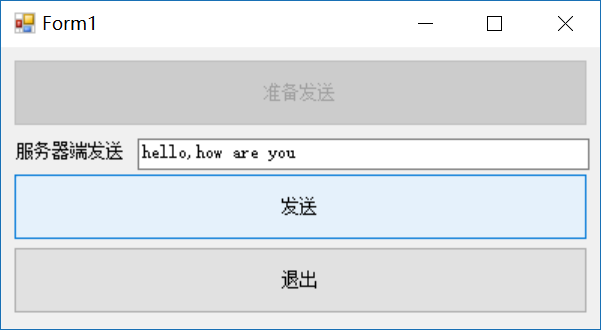
\includegraphics [width=0.5\textwidth]{figure//localserver.png}
	\caption{本地回环服务器端测试结果}\label{localserver}
\end{figure}

客户端:图\ref{localclient}
\begin{figure}[htbp]
	\centering
	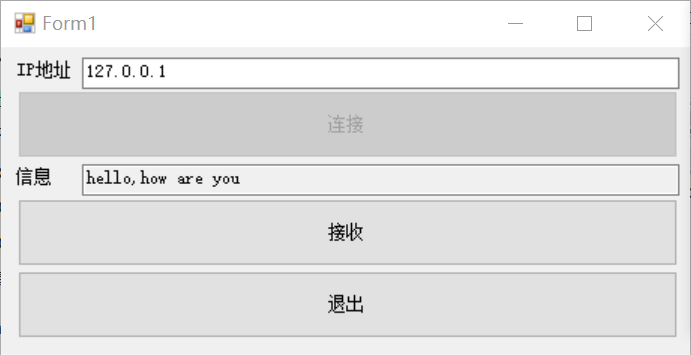
\includegraphics [width=0.5\textwidth]{figure//localclient.png}
	\caption{本地回环客户端测试结果}\label{localclient}
\end{figure}

\newpage
\subsection{远程互通IP记录}
主机1:图\ref{IP1}
\begin{figure}[htbp]
	\centering
	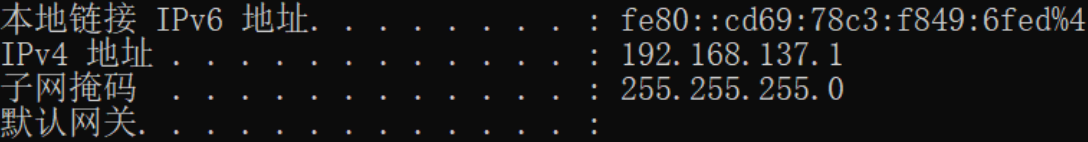
\includegraphics [width=1\textwidth]{figure//IP1.png}
	\caption{主机1IP}\label{IP1}
\end{figure}

主机2:图\ref{IP2}
\begin{figure}[htbp]
	\centering
	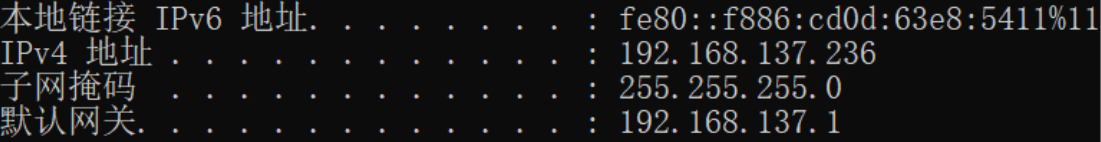
\includegraphics [width=1\textwidth]{figure//IP2.png}
	\caption{主机2IP}\label{IP2}
\end{figure}

\subsection{远程互通测试1结果(主机A做服务器端,主机B做客户端)}
主机1:图\ref{remote1local1}
\begin{figure}[htbp]
	\centering
	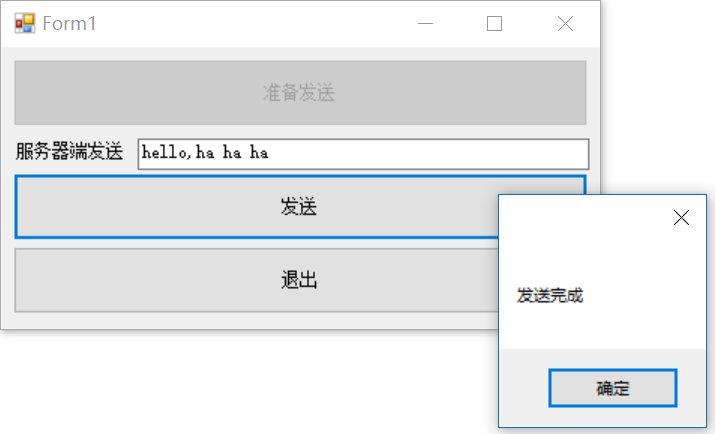
\includegraphics [width=0.5\textwidth]{figure//remote1local1.png}
	\caption{远程互通测试2主机2结果}\label{remote1local1}
\end{figure}

\newpage
主机2:图\ref{remote1local2}
\begin{figure}[htbp]
	\centering
	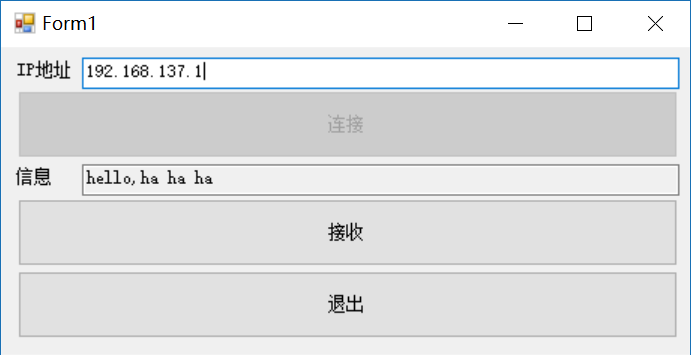
\includegraphics [width=0.5\textwidth]{figure//remote1local2.png}
	\caption{远程互通测试1主机1结果}\label{remote1local2}
\end{figure}

\subsection{远程互通测试2结果(主机A做客户端,主机B做服务器端)}
主机1:图\ref{remote2local1}
\begin{figure}[htbp]
	\centering
	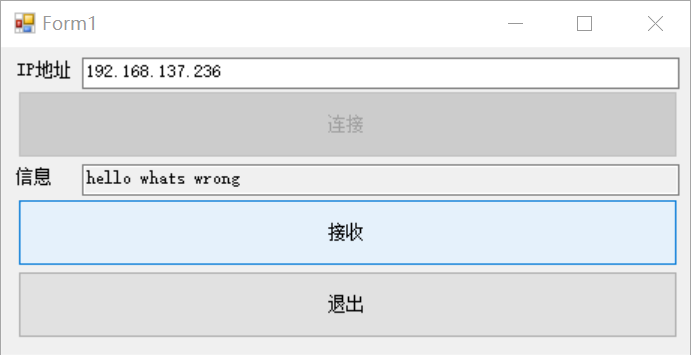
\includegraphics [width=0.5\textwidth]{figure//remote2local1.png}
	\caption{远程互通测试2主机1结果}\label{remote2local1}
\end{figure}

主机2:图\ref{remote2local2}
\begin{figure}[htbp]
	\centering
	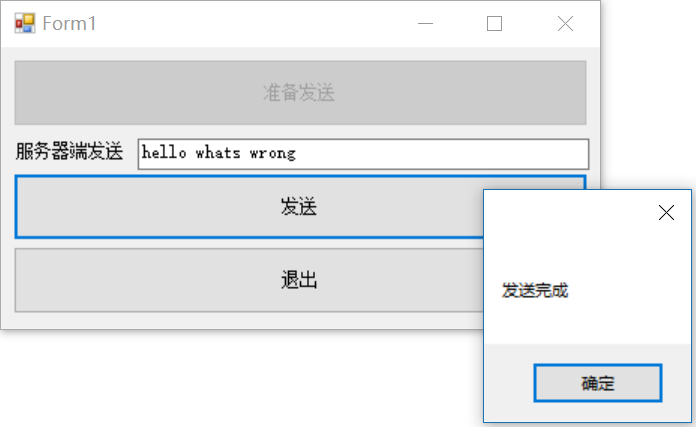
\includegraphics [width=0.5\textwidth]{figure//remote2local2.png}
	\caption{远程互通测试2主机2结果}\label{remote2local2}
\end{figure}

\end{spacing}
\section{问题及心得}
	\begin{itemize}
		\item 问题:在服务器端程序中,如果把服务器套接字的Socket.Close()调用放在发送完成后,则下一次开启监听时会报错。(图\ref{error})
		\begin{itemize}
			\item 原因:若在程序全部结束前调用了服务器套接字的Socket.Close(),服务器套接字将完全失效,此后必须对服务器套接字重新初始化才能进行其他操作。
			\item 解决:将服务器套接字的Socket.Close()调用放在窗口关闭后的主程序末尾。
		\end{itemize}
		\begin{figure}[htbp]
			\centering
			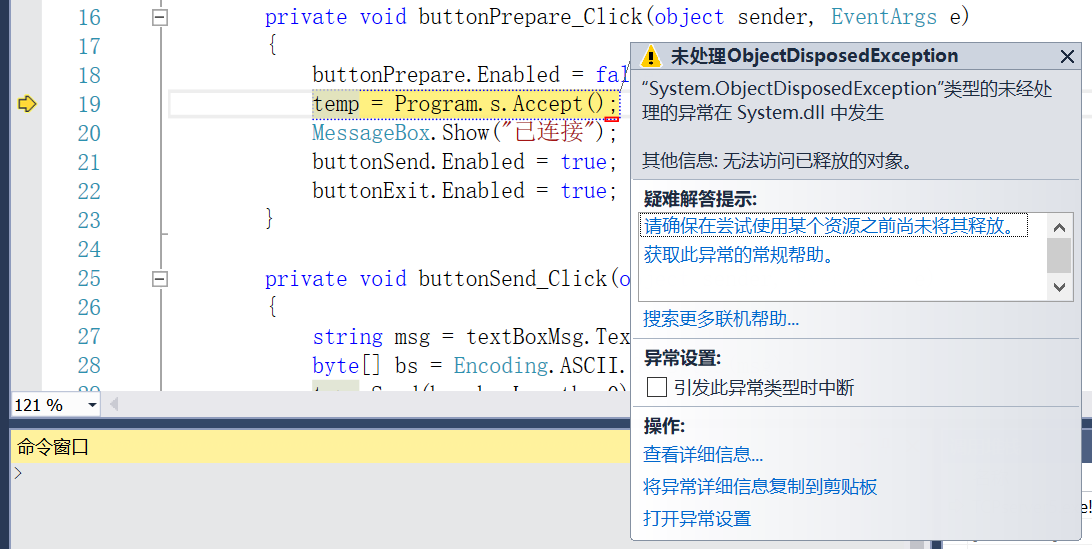
\includegraphics [width=0.5\textwidth]{figure//error.png}
			\caption{错误信息}\label{error}
		\end{figure}
		\item 心得:\begin{enumerate}
			\item 实践是检验真理的唯一标准;
			\item 实验是巩固知识的最快捷径;
			\item 掌握了C\#中TCP协议的使用方法;
			\item 明白了C\#Socket程序开发的一般模式;
			\item 精进了代码水平。
		\end{enumerate}
	\end{itemize}
\newpage
\titleformat{\chapter}{\heiti\Large}{附录~\Alph{chapter}}{11pt}{\Large}
\titlespacing{\chapter}{0pt}{*-4}{*4}
\renewcommand{\thechapter}{附录\Alph{chapter}.} 
\begin{appendix}
\chapter{核心代码清单}
\label{appendix}

\lstset{
	language={[Sharp]C},
	numbers=left,numberstyle=\tiny,
	basicstyle=\small\ttfamily,
	stringstyle=\color{codepurple},
	keywordstyle=\color{blue}\bfseries,
	commentstyle=\color{codegreen},
	frame=shadowbox,
	rulesepcolor=\color{codegray}
}

\section{TCPserver5/Program.cs}
\label{TCPserver5/Program.cs}
\begin{lstlisting}
using System;
using System.Windows.Forms;
using System.Net;
using System.Net.Sockets;

namespace TCPserver5
{
	static class Program
	{
		const int port = 2000;
		public static Socket s;
		/// <summary>
		/// 应用程序的主入口点。
		/// </summary>
		[STAThread]
		static void Main()
		{
			s = new Socket(AddressFamily.InterNetwork,
			 		SocketType.Stream,
			 		ProtocolType.Tcp);
			IPEndPoint ipe = new IPEndPoint(IPAddress.Any, port);
			//用指定的端口和ip初始化IPEndPoint类的新实例
			s.Bind(ipe);//绑定EndPoint对像(2000端口和ip地址)  
			s.Listen(0);//开始监听
			Application.EnableVisualStyles();
			Application.SetCompatibleTextRenderingDefault(false);
			Application.Run(new Form1());
			s.Close();
		}
	}
}
\end{lstlisting}

\section{TCPserver5/Form1.cs}
\label{TCPserver5/Form1.cs}
\begin{lstlisting}
using System;
using System.Text;
using System.Windows.Forms;
using System.Net.Sockets;

namespace TCPserver5
{
	public partial class Form1 : Form
	{
		Socket temp;
		public Form1()
		{
			InitializeComponent();
		}

		private void buttonPrepare_Click(object sender, EventArgs e)
		{
			buttonPrepare.Enabled = false;
			temp = Program.s.Accept();
			MessageBox.Show("已连接");
			buttonSend.Enabled = true;
			buttonExit.Enabled = true;
		}

		private void buttonSend_Click(object sender, EventArgs e)
		{
			string msg = textBoxMsg.Text;
			byte[] bs = Encoding.ASCII.GetBytes(msg);
			temp.Send(bs, bs.Length, 0);
			MessageBox.Show("发送完成");
		}


		private void buttonExit_Click(object sender, EventArgs e)
		{
			temp.Close();
			buttonSend.Enabled = false;
			buttonExit.Enabled = false;
			buttonPrepare.Enabled = true;
		}
	}
}

\end{lstlisting}

\section{TCPclient5/Program.cs}
\label{TCPclient5/Program.cs}
\begin{lstlisting}
using System;
using System.Collections.Generic;
using System.Linq;
using System.Threading.Tasks;
using System.Windows.Forms;

namespace TCPclient5
{
	static class Program
	{
		/// <summary>
		/// 应用程序的主入口点。
		/// </summary>
		[STAThread]
		static void Main()
		{
			Application.EnableVisualStyles();
			Application.SetCompatibleTextRenderingDefault(false);
			Application.Run(new Form1());
		}
	}
}
\end{lstlisting}

\section{TCPclient5/Form1.cs}
\label{TCPclient5/Form1.cs}
\begin{lstlisting}
using System;
using System.Text;
using System.Windows.Forms;
using System.Net;
using System.Net.Sockets;

namespace TCPclient5
{
	public partial class Form1 : Form
	{
		Socket c;
		const int port = 2000;
		public Form1()
		{
			InitializeComponent();
		}

		private void buttonConnect_Click(object sender, EventArgs e)
		{
			string ip_str = textBoxIP.Text;
			IPEndPoint ipe = new IPEndPoint(IPAddress.Parse(ip_str), port);
			c = new Socket(AddressFamily.InterNetwork,
					SocketType.Stream,
					ProtocolType.Tcp);//创建Socket
			c.Connect(ipe);
			MessageBox.Show("连接成功");
			buttonConnect.Enabled = false;
			buttonRecv.Enabled = true;
			buttonExit.Enabled = true;
		}

		private void buttonRecv_Click(object sender, EventArgs e)
		{
			buttonRecv.Enabled = false;
			byte[] recvBytes = new byte[1024];
			int bytes = c.Receive(recvBytes, recvBytes.Length, 0);
			//从服务器端接受返回信息
			textBoxRecv.Text = Encoding.ASCII.GetString(recvBytes, 0, bytes);
			buttonRecv.Enabled = true;
		}

		private void buttonExit_Click(object sender, EventArgs e)
		{
			c.Close();
			buttonConnect.Enabled = true;
			buttonRecv.Enabled = false;
			buttonExit.Enabled = false;
		}
	}
}
\end{lstlisting}
\end{appendix}
\end{document}